\documentclass[12pt,a4paper]{article}
\usepackage{graphicx}
\begin{document}
	\begin{titlepage}
		\centering
		\vspace*{\fill}
		
		\vspace*{0.5cm}
		
		\huge\bfseries
		\rule{\textwidth}{1.6pt}\\[\baselineskip]
		Thutong Site Learning Center User Manual
		
		\vspace*{0.5cm}
		
		\large Contributors: \\[\baselineskip]
		
			{Fiwa Lekhulani\\Daniel Rocha\\lebogang Ntatleng\\Lesego Mabe\\Tlou Lebelo\\Oluwatosin Botti}
		
		\rule{\textwidth}{1.6pt}\\[\baselineskip]
		
		
		\vspace*{\fill}
	\end{titlepage}


	\date{\textbf{\today}}
	\pagenumbering{roman}
	%\noindent\rule{\textwidth}{1pt}
	\pagebreak
	\tableofcontents
	\newpage
	\pagenumbering{arabic}

s

	\section{Product Overview}
		The Thutong Site Learning Centre is an online learning system intended for high school students. It is aimed at providing students with online material to learn or catch up on any academic content that they might have missed in class or did not comprehend during class. it is also aimed at providing teachers a way of uploading academic content to the system for students to learn from and provide quizzes for the students to test their knowledge after the completion of a topic. 
	
	\section{System Configuration}
		The Thutong Site Learning Centre does need not be installed on any any digital device, as it is available online. The system can be accessed through desktop computers and mobile devices and users will need a network connection and mobile data in order to huse the learning centre 
		
		%NOTE:please load an image here!!!
		
	\section{Getting Started}
		The Thutong Learning Centre is aimed at improving South Africa's pass rate; it intendeds to be used by every student in South Africa to improve their understand and envitably pass. It is free and no license is needed to use it to enable more students to have access to it.\\
		There Thutong Learning Centre encompasses four types of users:
		\begin{itemize}
			\item Students
			\item Expert Consultants(Teachers)
			\item Marketing Consultants
			\item Administrator
		\end{itemize} 
		  
		\subsection{The student}
		 This student is able to login with either their google, facebook or email account in order to have personalized access when using the learning centre. The student is also able to search for a specific subject and be able to view content within that subject (regardless of their login status). Figure 1 shows the login page where the user will fill in their created account details to access the system. Figure 2 shows the registration form required to filled by new users\\
		 
		 %imagee to be loaded here(screenshot)
		 
		 \begin{figure}
		 	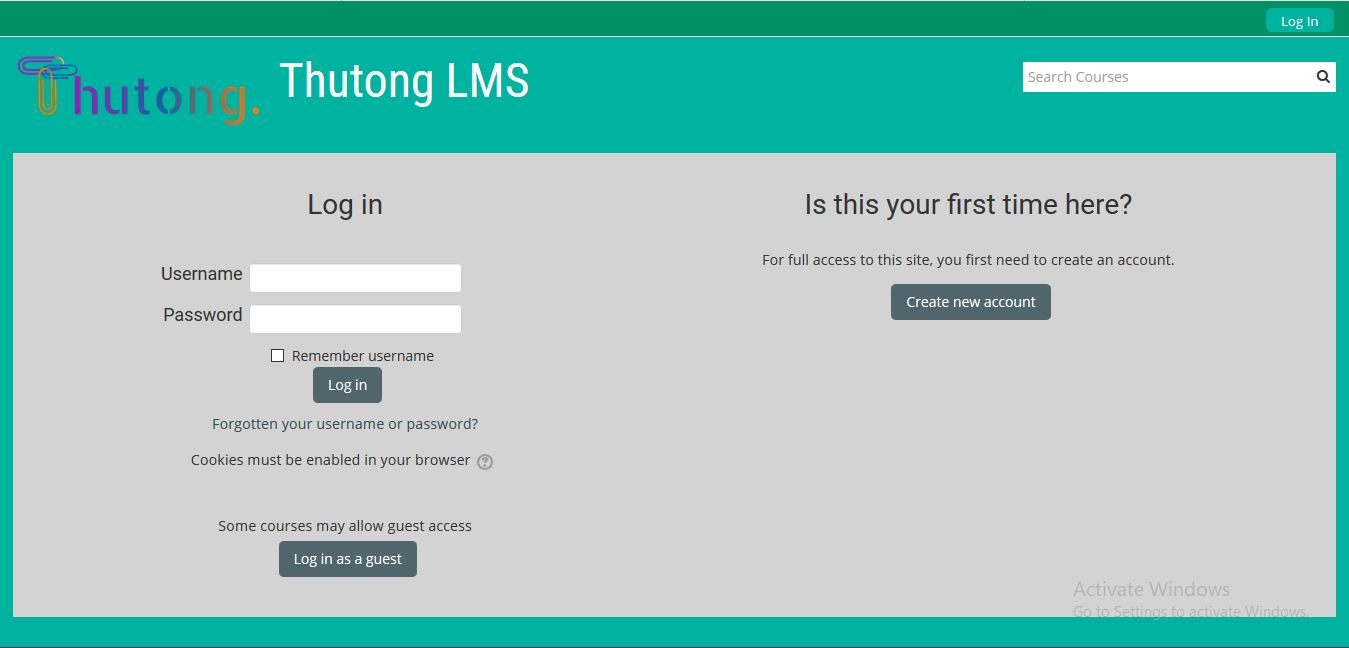
\includegraphics[width=\linewidth]{login.JPG}
		 	\caption{User Login.}
		 	\label{fig:user login}
		 \end{figure}
		 
		 \begin{figure}
		 	\includegraphics[width=\linewidth]{Register.JPG}
		 	\caption{User Registration.}
		 	\label{fig:user registration}
		 \end{figure}
		 
		 \subsection{The Expert Consultant}
		 The Expert consultant needs to be able to, other than logging in, add academic content intended for students. They should also be able to create quizzes for students and be able to remove all of the above-mentioned entities.
		
		\subsection{The Marketing Consultant}
		 This user needs to be able to add, remove and update marketing content within the system such as vacancies, advertisements and donation request.
		 
		 
		 \subsection{The Administrator}
		 Also known as the superuser, this user will have all the access to all users profilesbeing able to removed those deemed to use the learing cenre inappropriately. Admin will also be responsible for the aapproval, addition, validation and removal of Expert and Marketing consultant accounts.
		 
	\section{Using the System}
	 This section discusses how to go about using various functions of the learning system.
	 	\subsection{Home Page}
		This page is the first page a user sees when they access the Thutong Learning Centres' web page. Here they have the options to search topiccs and subject lessons, login, read more about the online centre or view grades. This is the page that navigates to all other functions of 
		
		\begin{figure}
		 	\includegraphics[width=\linewidth]{Home.JPG}
		 	\caption{Home Page}
		 	\label{fig: Home Page}
		 \end{figure}
		 
	 	\subsection{Login}
	 	 As mentioned in 4.1 and Figure 1 when the user chooses to login from the home page they will see figure 1 and beyond completing the necessary details and their account is verified they will be logged in and rediercted to the homepage. 
	 	 
	 	 \subsection{Search}
	 	 When searching the user types in the relevant item they would like t find and they select what criteria it falls into  by selecting on the "search by" dropdown and then click submit. They will be redirected to thepage that retrieves all content related to their search.
		  \begin{figure}
		 	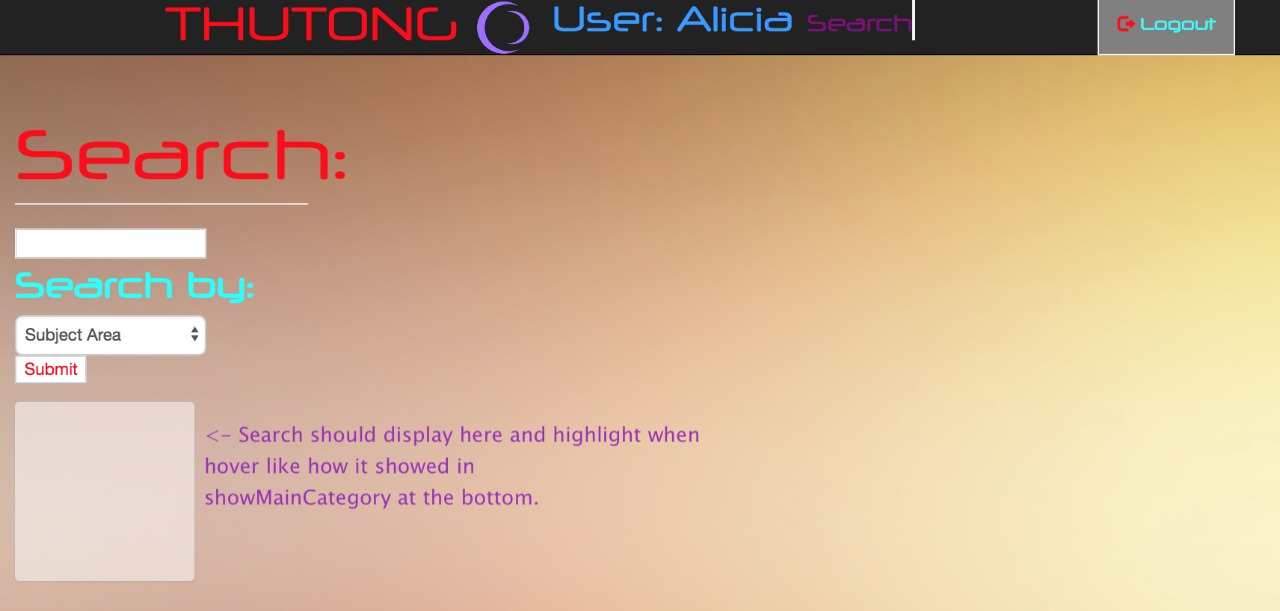
\includegraphics[width=\linewidth]{Search.png}
		 	\caption{Search}
		 	\label{fig: Search}
		 \end{figure}
	 	
	 	 \subsection{Grade and Subject Selection}
		 Upon selecting the "Grades" on the home page they will be directed to the page illustrated by Figure *. From this page a learner selects a their appropriate grade, then being redirected to Figure *, the grades' subject list page.
		 \newline
		 From the subject list page the  user selects a subject either Mathematics, Accounting, Physical and Life Sciences. Upon selecting their preferred subject they want to do then they will be redirected to Figure * where they will see a specific topic from the choosen subject.
		 
		 begin{figure}
		 	\includegraphics[width=\linewidth]{Grades.JPG}
		 	\caption{Grade}
		 	\label{fig: Grades}
		 \end{figure}
		 
		 begin{figure}
		 	\includegraphics[width=\linewidth]{subjects.JPG}
		 	\caption{Subjects}
		 	\label{fig: Subjects}
		 \end{figure}
		 
		 begin{figure}
		 	\includegraphics[width=\linewidth]{SubjectTopics.JPG}
		 	\caption{Topics}
		 	\label{fig: Topics}
		 \end{figure}
	 	 
	 	 \subsection{Viewing course content}
		After selecting a topic from Figure * the user is redirected to a lesson where they can view documents or videos related to the stipulated heading, this is shown in Figure *.
		
		begin{figure}
		 	\includegraphics[width=\linewidth]{Lesson.JPG}
		 	\caption{PDF Lesson}
		 	\label{fig: PDF Lesson}
		 \end{figure}
		
		\subsection{Completing a quiz}
		After completing a lesson, the user has the option to do a quiz about the specific lesson they've just completed. Once complete the user selects "submit" and thereafter a mark at the bottom of the page. This mark wil be stored to the users' profile.
		%begin{figure}
		 	%\includegraphics[width=\linewidth]{Quiz.JPG}
		 	%\caption{Quiz}
		 	%\label{fig: Quiz}
		 %\end{figure}
	
\end{document}
